% !TEX TS-program = pdflatex
% !TEX encoding = UTF-8 Unicode

% This file is a template using the "beamer" package to create slides for a talk or presentation
% - Giving a talk on some subject.
% - The talk is between 15min and 45min long.
% - Style is ornate.

% MODIFIED by Jonathan Kew, 2008-07-06
% The header comments and encoding in this file were modified for inclusion with TeXworks.
% The content is otherwise unchanged from the original distributed with the beamer package.

\documentclass{beamer}
\setbeamercovered{invisible}



% Copyright 2004 by Till Tantau <tantau@users.sourceforge.net>.
%
% In principle, this file can be redistributed and/or modified under
% the terms of the GNU Public License, version 2.
%
% However, this file is supposed to be a template to be modified
% for your own needs. For this reason, if you use this file as a
% template and not specifically distribute it as part of a another
% package/program, I grant the extra permission to freely copy and
% modify this file as you see fit and even to delete this copyright
% notice. 


\mode<presentation>
{
  \usetheme{Warsaw}
  % or ...

  % or whatever (possibly just delete it)
}


\usepackage[english]{babel}
% or whatever

\usepackage[utf8]{inputenc}
\usepackage{qrcode}
\usepackage{hyperref}
\usepackage{ytableau}
\usepackage{longtable}
% or whatever

\usepackage{times}
\usepackage[T1]{fontenc}
% Or whatever. Note that the encoding and the font should match. If T1
% does not look nice, try deleting the line with the fontenc.

%%% MATH RELATED

\title{MATH 180 Strategies of Problem Solving} 
\subtitle
{} % (optional)

\author[W.R. Casper] % (optional, use only with lots of authors)
{W.R. Casper}
% - Use the \inst{?} command only if the authors have different
%   affiliation.

\institute[California State University Fullerton] % (optional, but mostly needed)
{
  Department of Mathematics\\
  California State University Fullerton}
% - Use the \inst command only if there are several affiliations.
% - Keep it simple, no one is interested in your street address.

\subject{Talks}
% This is only inserted into the PDF information catalog. Can be left
% out. 



% If you have a file called "university-logo-filename.xxx", where xxx
% is a graphic format that can be processed by latex or pdflatex,
% resp., then you can add a logo as follows:

% \pgfdeclareimage[height=0.5cm]{university-logo}{university-logo-filename}
% \logo{\pgfuseimage{university-logo}}



% Delete this, if you do not want the table of contents to pop up at
% the beginning of each subsection:
\AtBeginSubsection[]
{
  \begin{frame}<beamer>{Outline}
    \tableofcontents[currentsection,currentsubsection]
  \end{frame}
}


% If you wish to uncover everything in a step-wise fashion, uncomment
% the following command: 

%\beamerdefaultoverlayspecification{<+->}


\begin{document}

\begin{frame}
  \titlepage
\end{frame}

\begin{frame}{Outline}
  \tableofcontents
  % You might wish to add the option [pausesections]
\end{frame}

% Since this a solution template for a generic talk, very little can
% be said about how it should be structured. However, the talk length
% of between 15min and 45min and the theme suggest that you stick to
% the following rules:  

% - Exactly two or three sections (other than the summary).
% - At *most* three subsections per section.
% - Talk about 30s to 2min per frame. So there should be between about
%   15 and 30 frames, all told.

\section{SoPS Lecture 8}

\subsection{Last time}


\begin{frame}{Review}
  \begin{block}{Last time}
    \begin{itemize}
\pause
      \item we played Break the Cube
\pause
      \item we talked about proofs
\pause
      \item we constructed a Break the Cube: Solitaire puzzle
    \end{itemize}
  \end{block}
\end{frame}

\subsection{Sprouts}

\begin{frame}{Sprouts by John Conway}
  \begin{block}{Rules}
    
    \begin{itemize}
\pause
      \item draw a few starting seeds
\pause
      \item each turn a player must
        \begin{itemize}
          \item \textbf{sprout} a vine between two seeds
          \item \textbf{spawn} a new seed along the vine 
        \end{itemize}
      \item restrictions
        \begin{itemize}
          \item \textbf{no overlaps}: vines cannot cross
          \item \textbf{no overflow}: seeds can have at most 3 vines attached
        \end{itemize}
\pause
      \item first player unable to sprout loses
    \end{itemize}
  \end{block}
\end{frame}
 
\begin{frame}{Two-seed game example}
  \begin{center}
    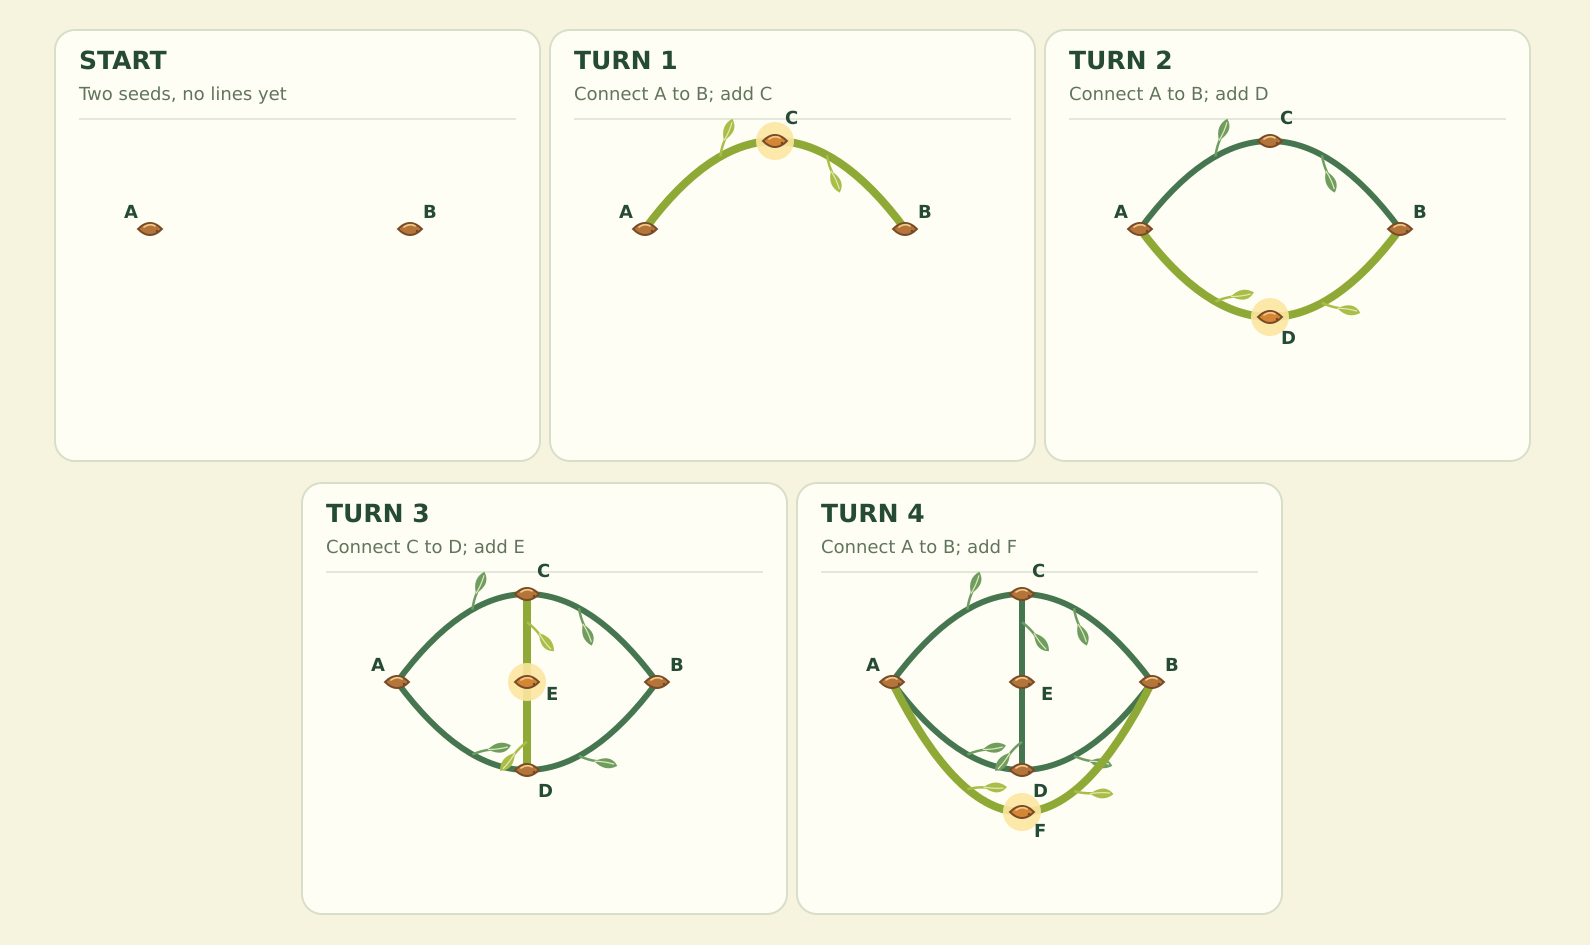
\includegraphics[width=\linewidth]{fig/sprouts-two-seeds}
  \end{center}
\end{frame}

\begin{frame}{No overlaps}
  \begin{center}
    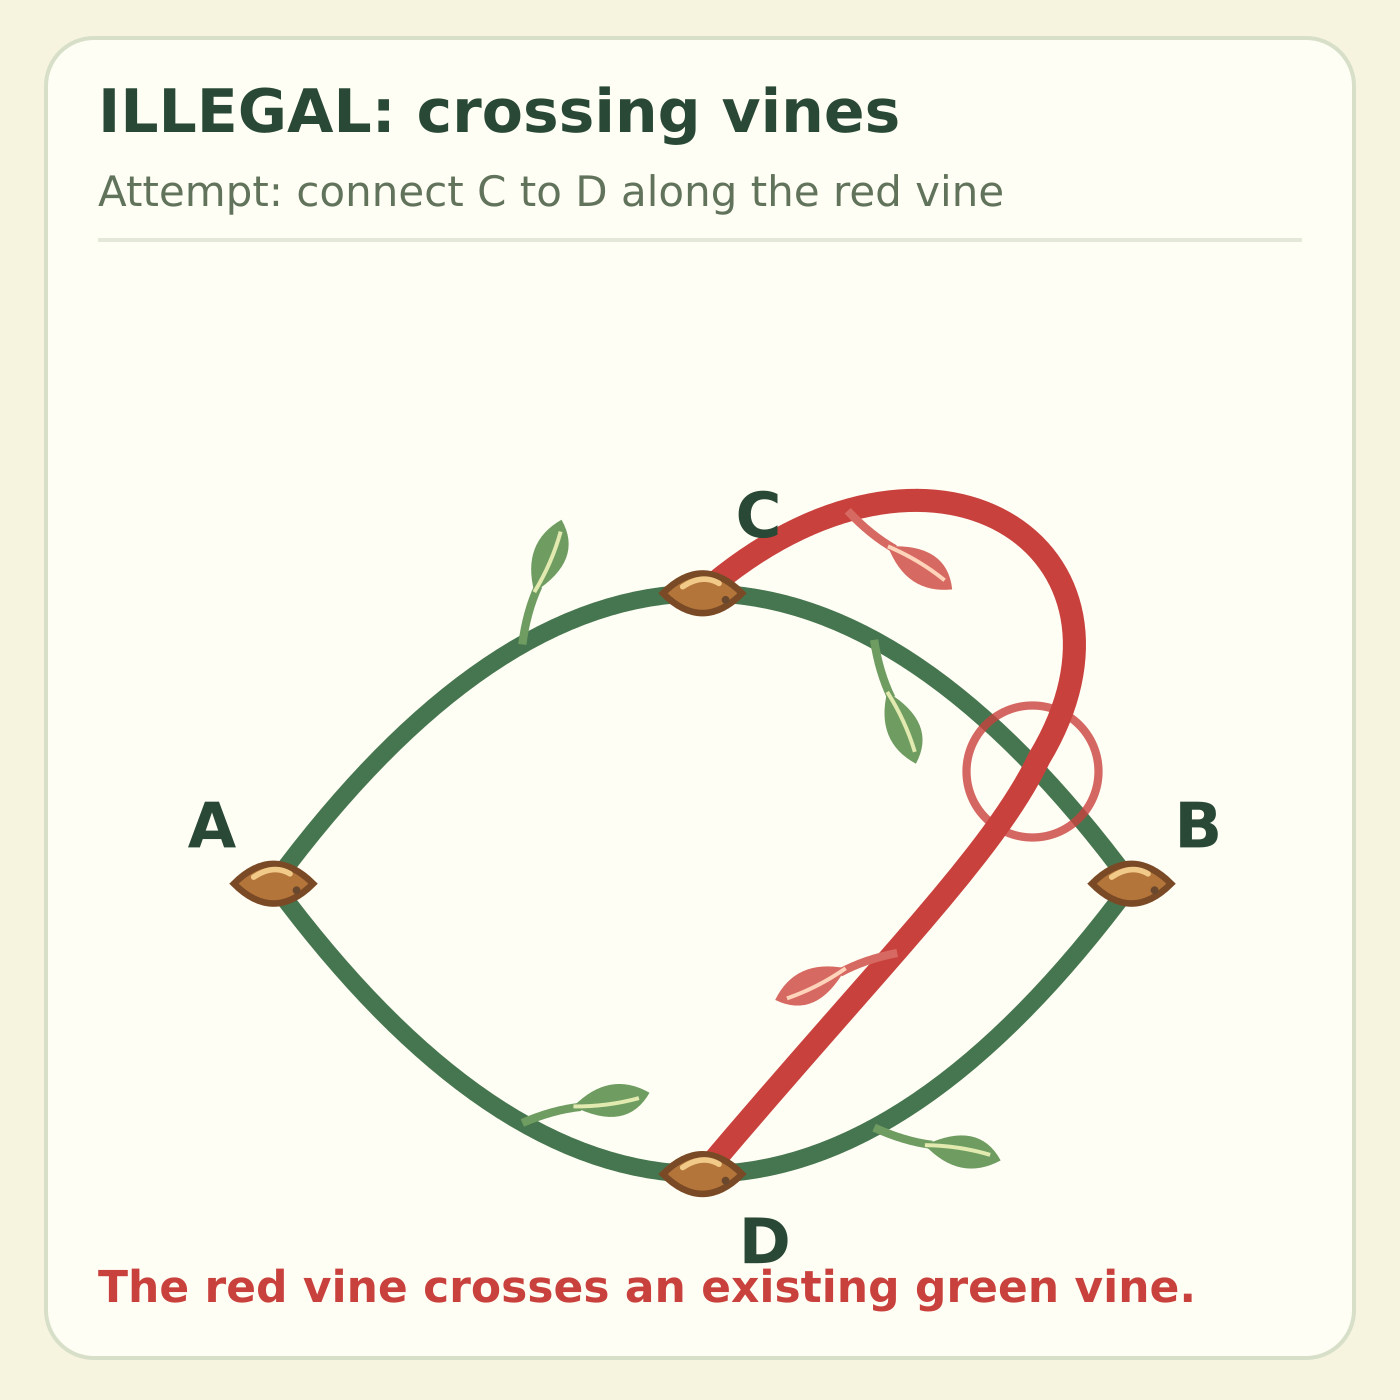
\includegraphics[width=0.5\linewidth]{fig/illegal-sprouts-crossing}
  \end{center}
\end{frame}

\begin{frame}{No overflow}
  \begin{center}
    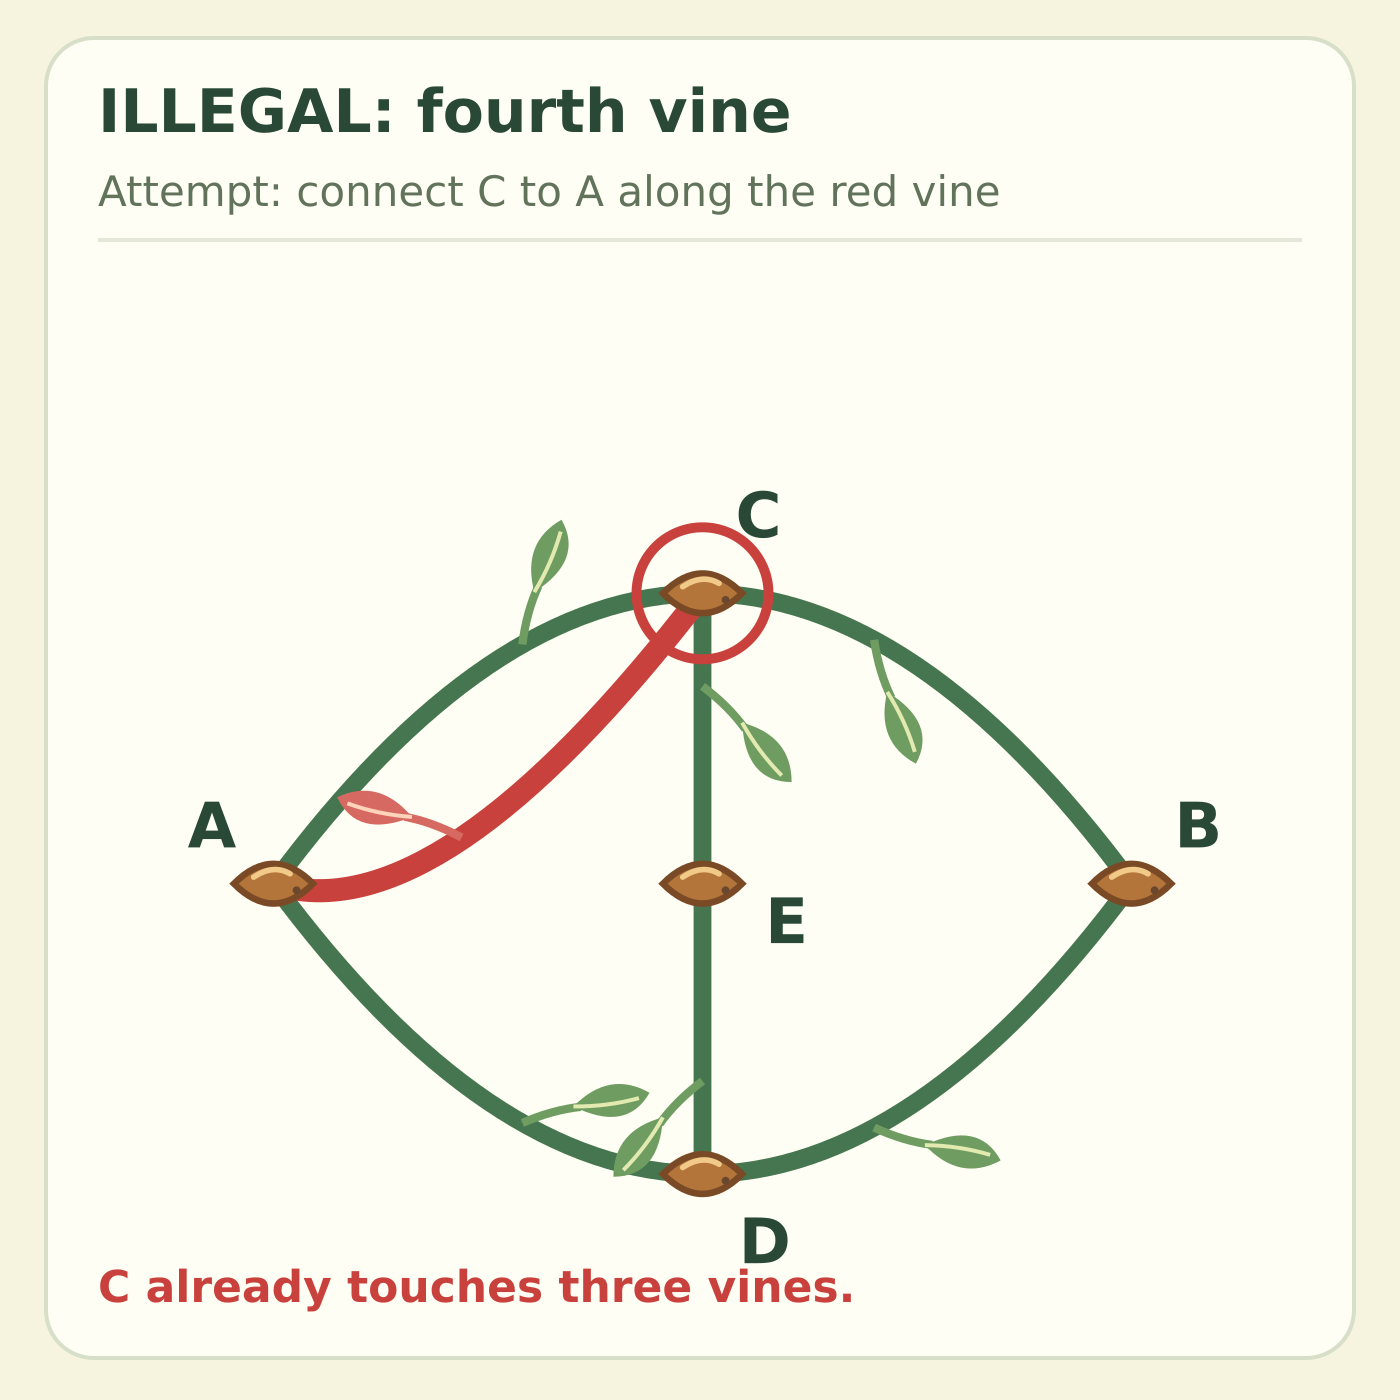
\includegraphics[width=0.5\linewidth]{fig/illegal-sprouts-fourth-vine}
  \end{center}
\end{frame}

\begin{frame}{Let's play!}
  \begin{block}{Activity}
    \begin{itemize}
\pause
      \item play a game of sprouts with $3-6$ starting seeds
\pause
      \item {\color{red}record}: number of starting seeds, number of seeds at end
\pause
      \item think of an interesting question to ask about the game
    \end{itemize}
  \end{block}
\end{frame}

\begin{frame}{Questions}
\pause
  \begin{block}{Question 1}
    Can you tell from the final number of seeds how many turns were taken?
  \end{block}
\pause
  \begin{block}{Question 2}
    Does the game always have to end?
  \end{block}

\end{frame}

\subsection{Graph theory}
 
\begin{frame}{Graphs}
\pause
  \begin{block}{Definition}
    A \textbf{graph} or \textbf{network} is a a collection of points called \textbf{vertices} or \textbf{nodes} connected together by curve segements that we call \textbf{edges}.
  \end{block}
\pause
  \textbf{Examples:}
  \begin{itemize}
\pause
    \item sprout games make graphs!
\pause
    \item social networks
\pause
    \item linked pages on Wikipedia
\pause
    \item aviation/flight networks
  \end{itemize}
\end{frame}

\begin{frame}{Social network}
  \begin{center}
    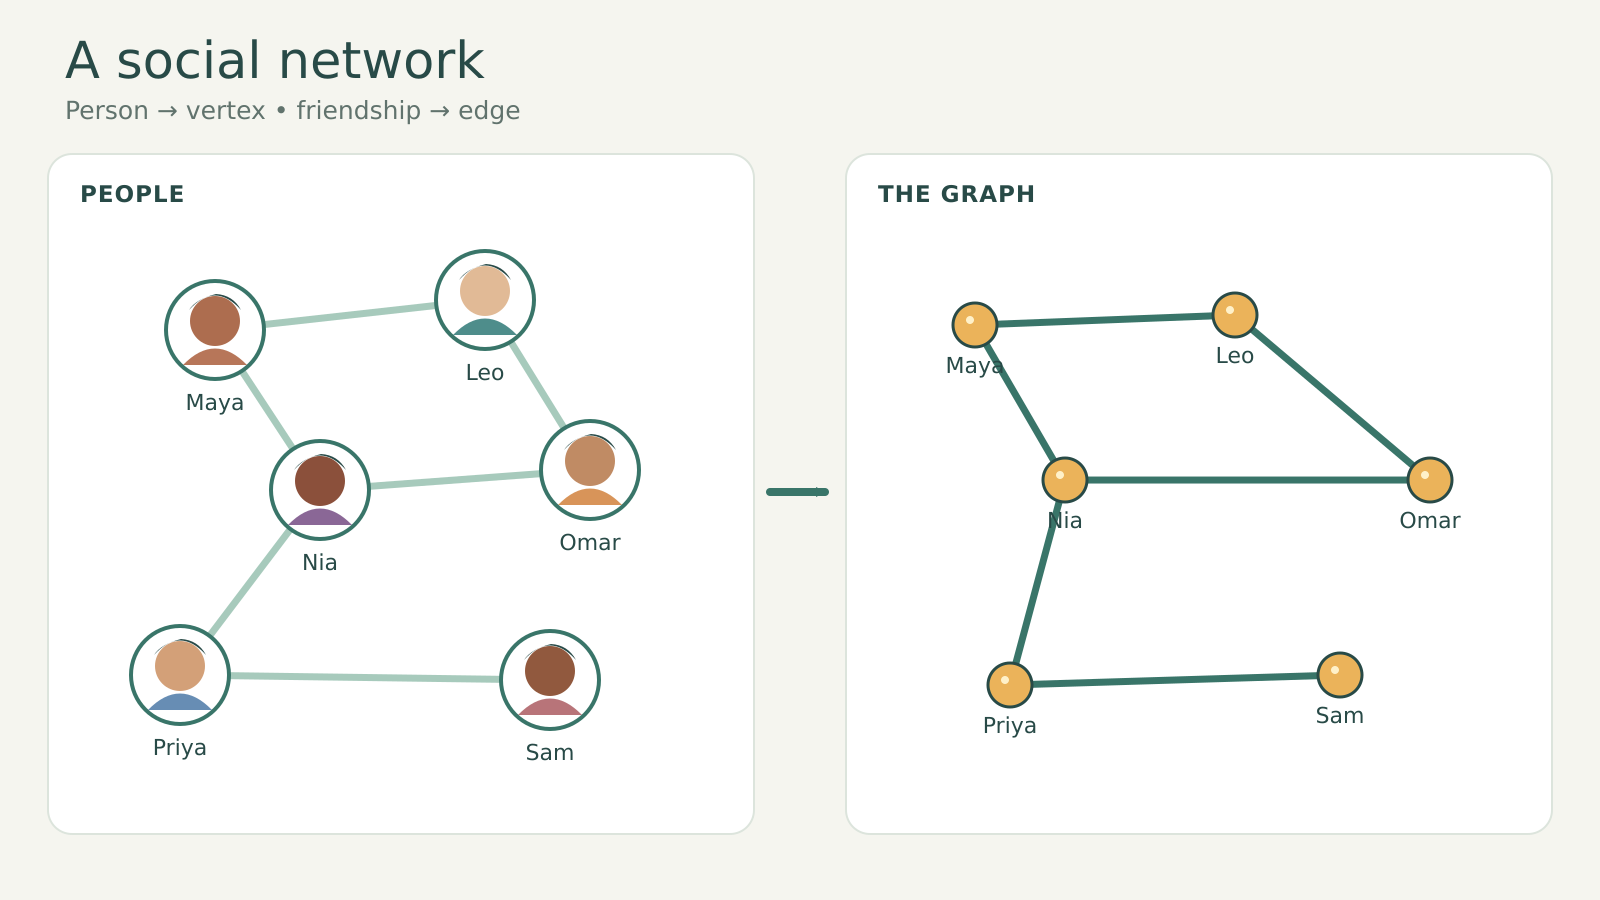
\includegraphics[width=0.9\linewidth]{fig/graph-application-social}
  \end{center}
\end{frame}

\begin{frame}{Wikipedia articles}
  \begin{center}
    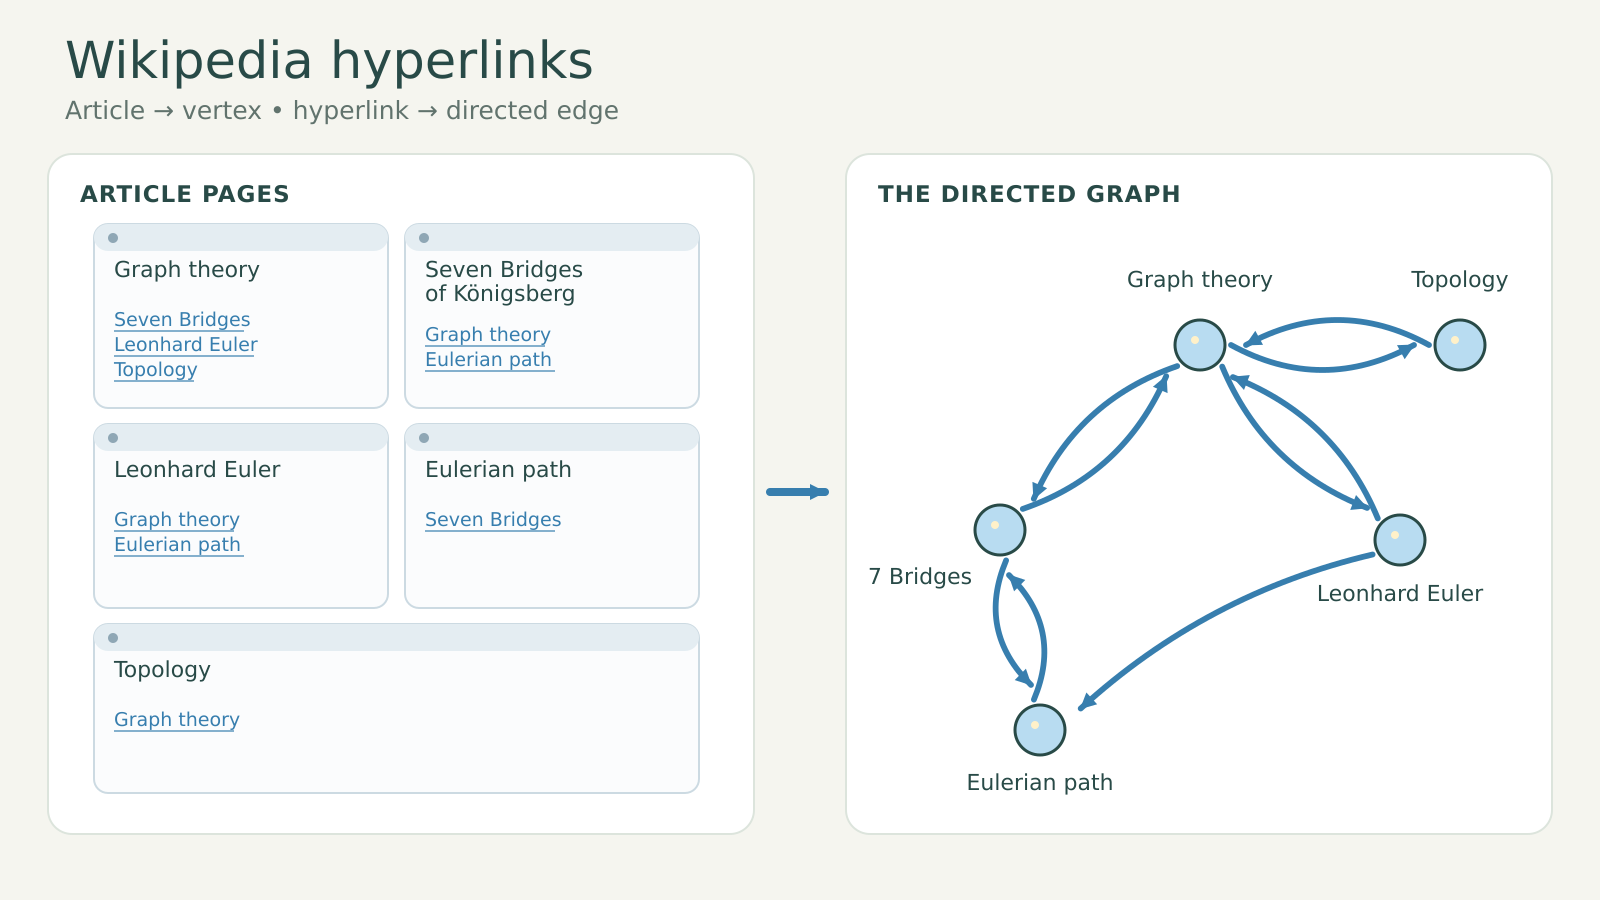
\includegraphics[width=0.9\linewidth]{fig/graph-application-wikipedia}
  \end{center}
\end{frame}

\begin{frame}{Direct flights}
  \begin{center}
    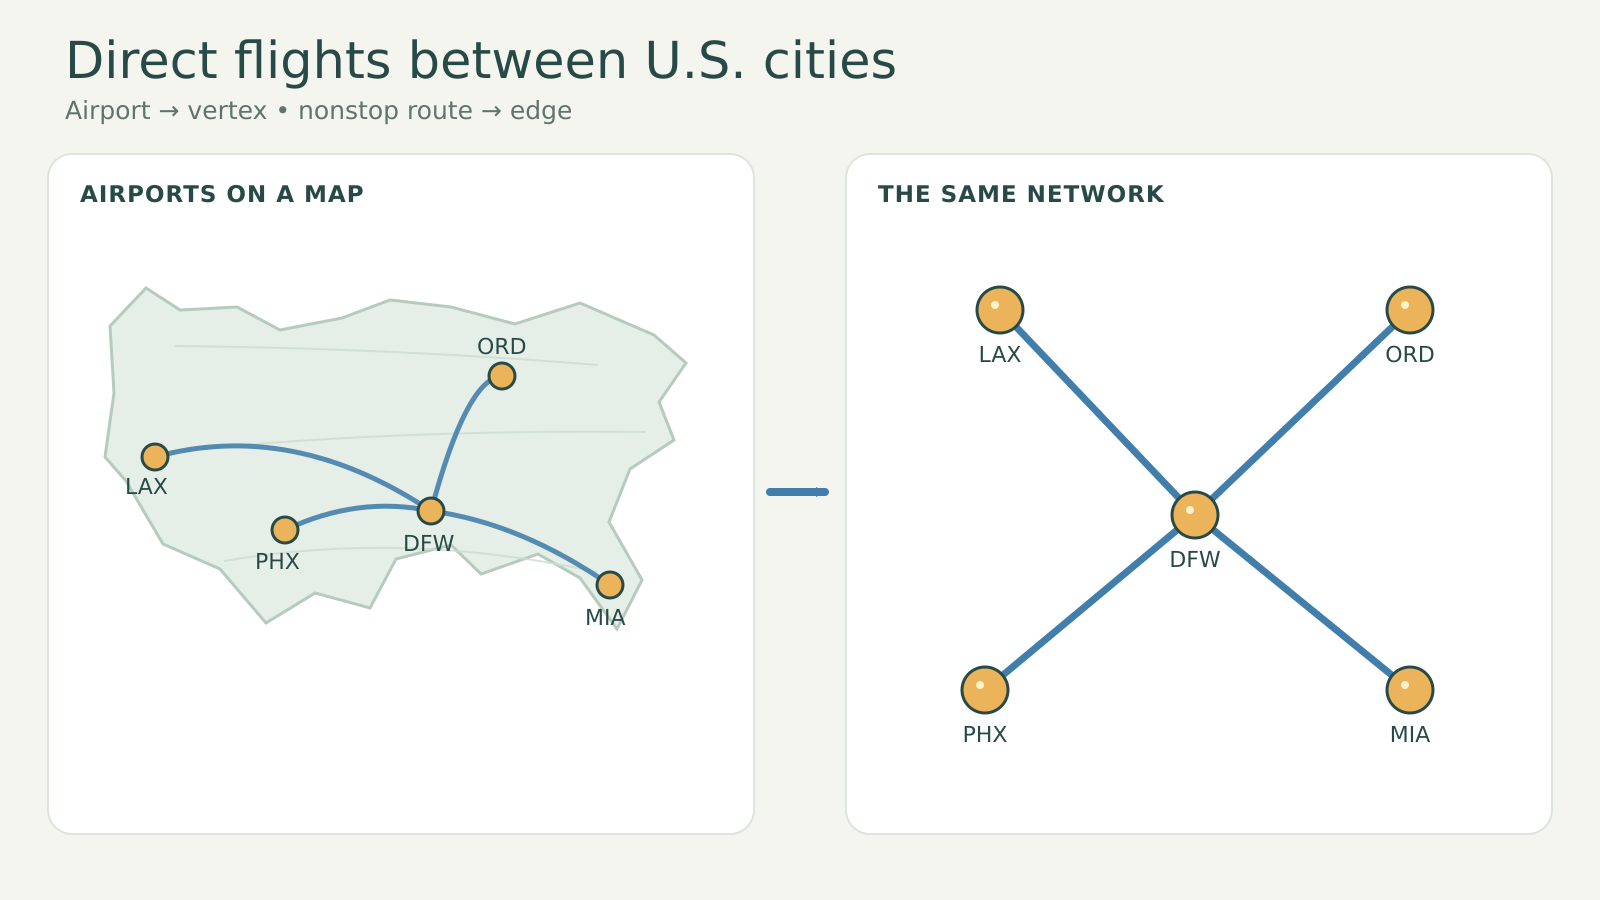
\includegraphics[width=0.9\linewidth]{fig/graph-application-flights}
  \end{center}
\end{frame}

\begin{frame}{Zoo of graphs}
  \begin{center}
    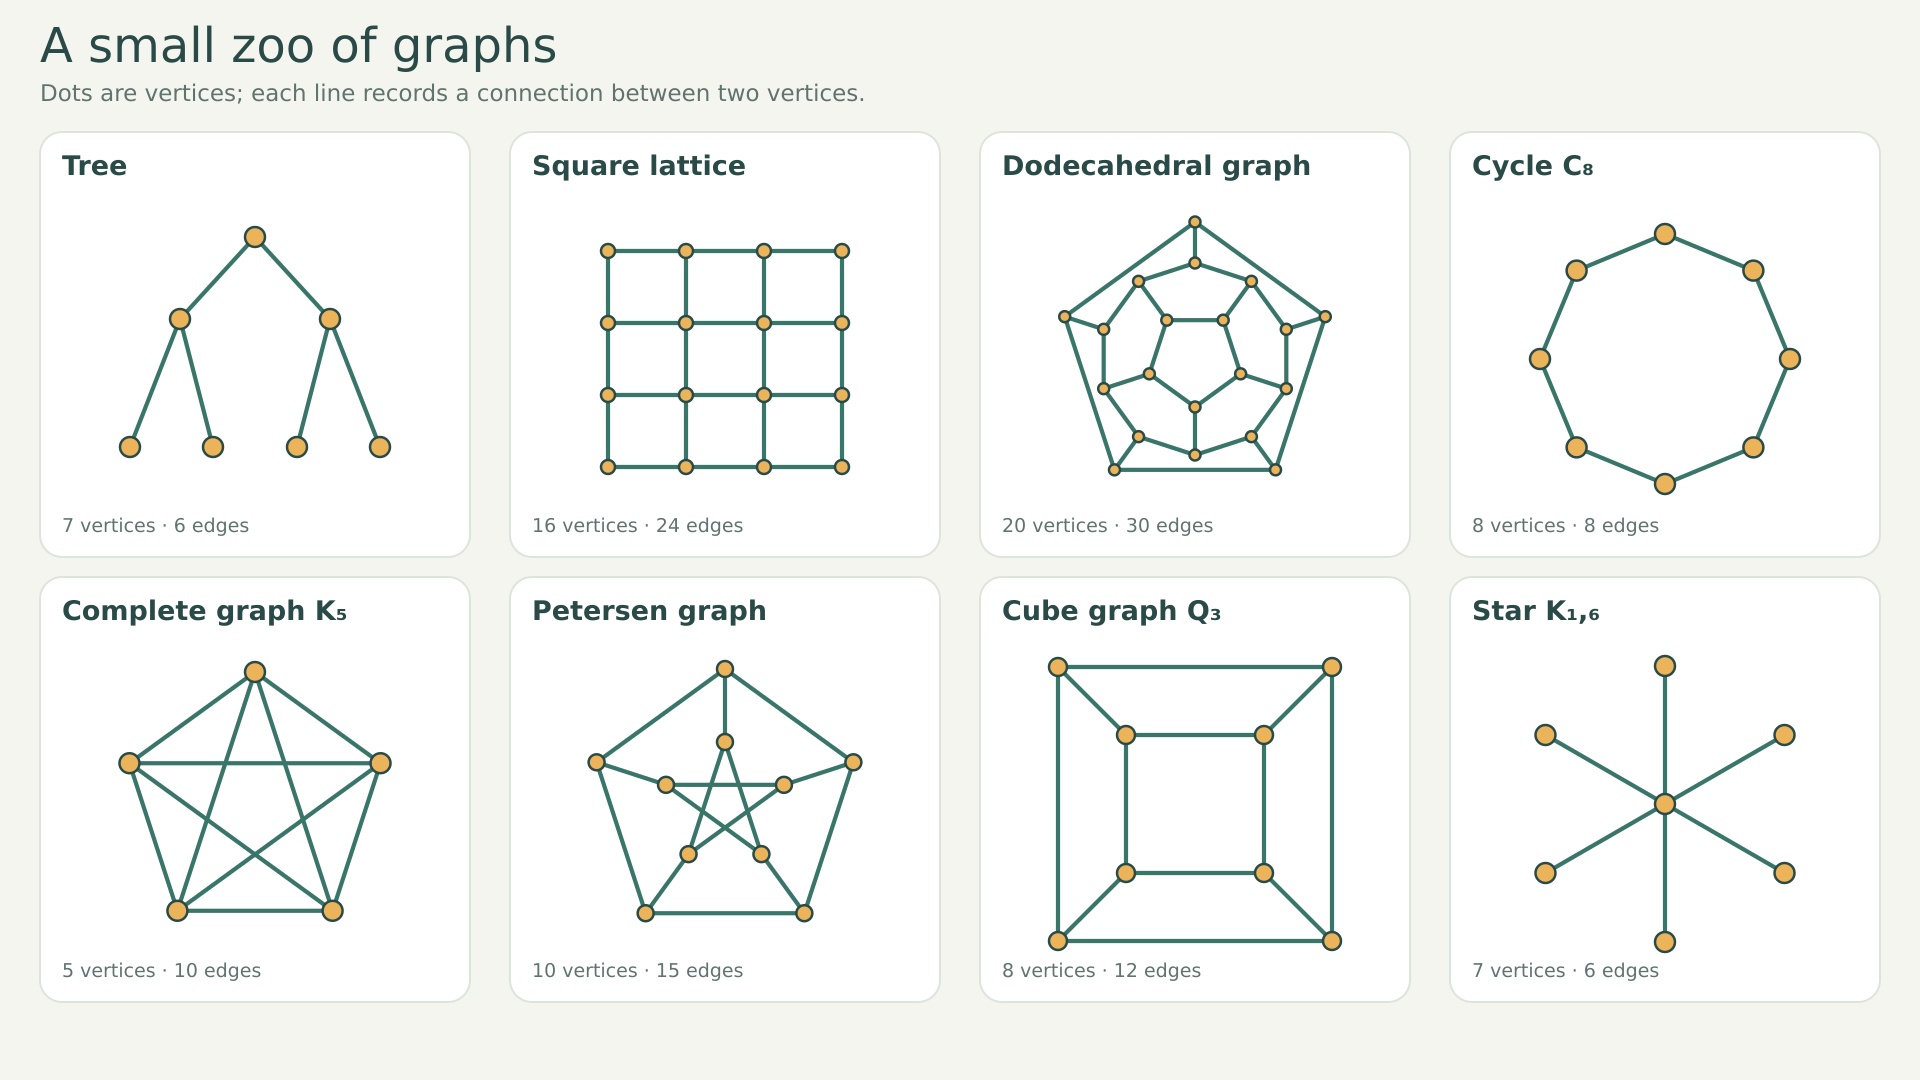
\includegraphics[width=0.9\linewidth]{fig/graph-zoo}
  \end{center}
\end{frame}


\begin{frame}{Properties of sprout graphs}
\pause
  \begin{block}{Question}
    Can we tell if a particular graph came from a game of Sprouts?  What properties should it have?
  \end{block}
\pause
  \begin{block}{Definition}
    The \textbf{degree} of a vertex is how many edges are coming out of it.
  \end{block}
\pause
  \begin{block}{Definition}
    A graph is called \textbf{planar} if no edges in the graph overlap.
  \end{block}
\end{frame}

\begin{frame}{Planar graphs}
  \begin{center}
    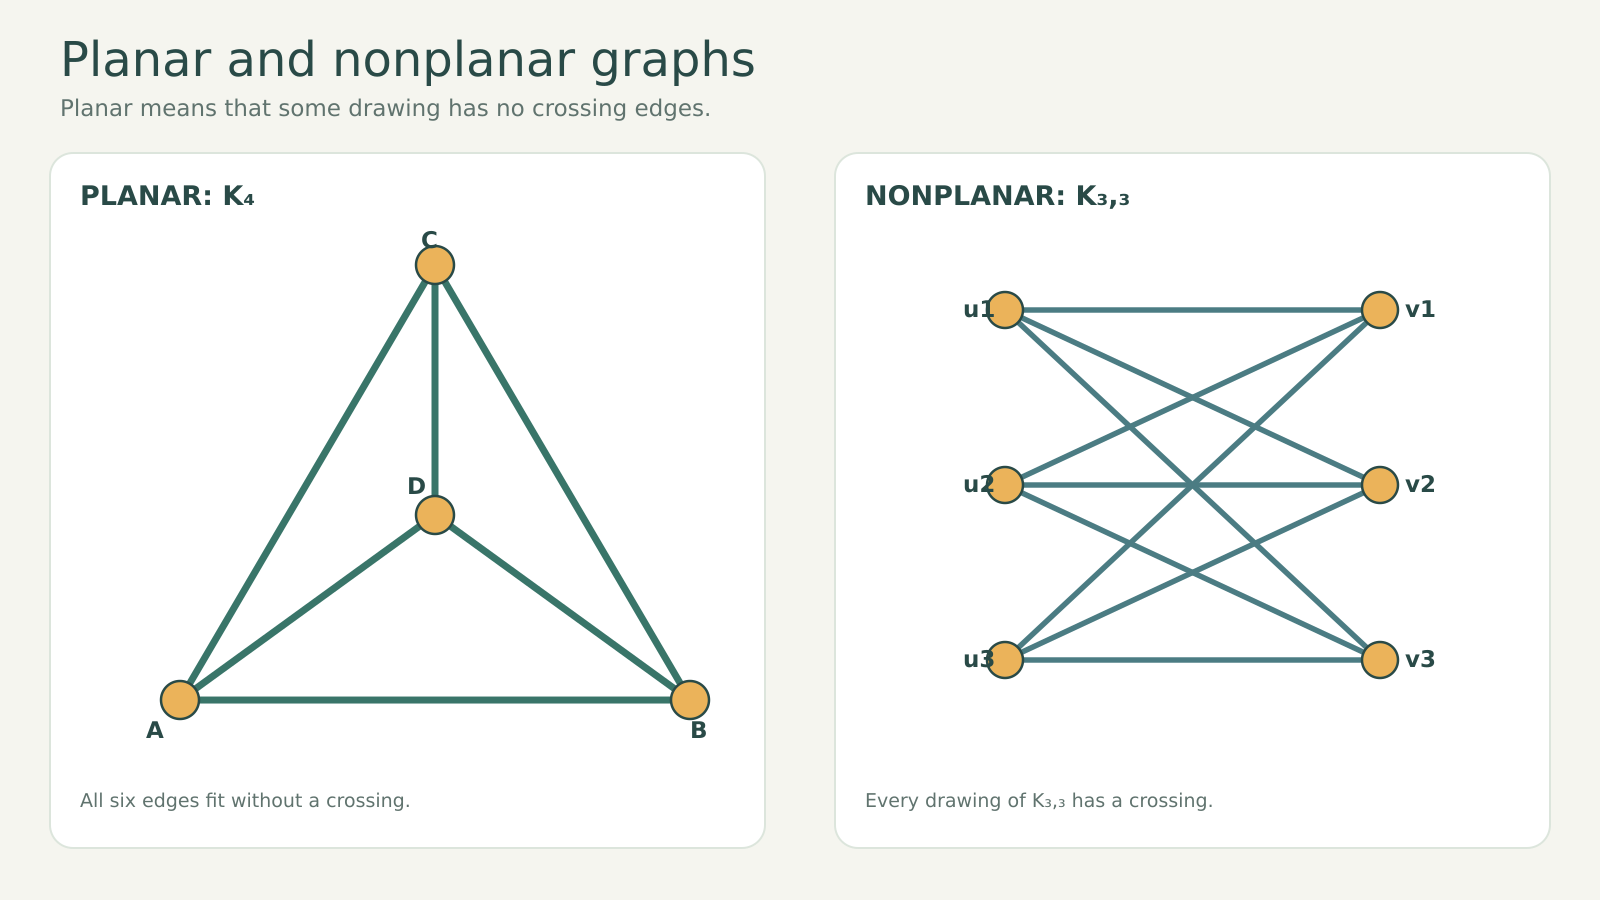
\includegraphics[width=0.9\linewidth]{fig/graph-planarity}
  \end{center}
\end{frame}

\begin{frame}{Vertex degree}
  \begin{center}
    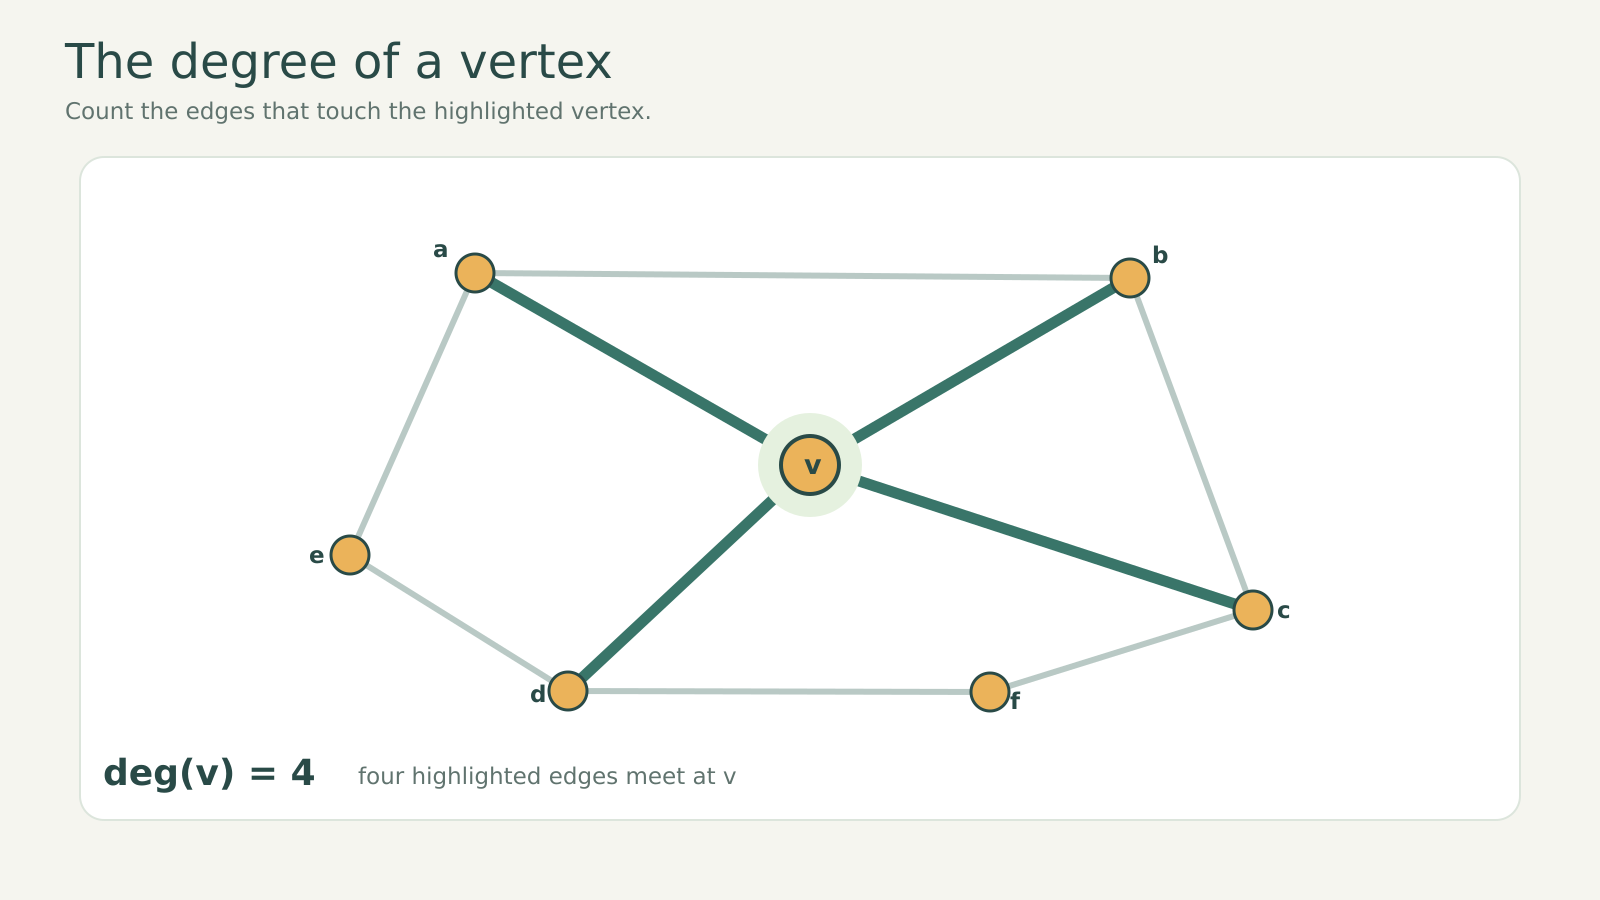
\includegraphics[width=0.9\linewidth]{fig/graph-vertex-degree}
  \end{center}
\end{frame}

\subsection{Sprout puzzles}

\begin{frame}{Longest game}
  \begin{block}{Activity:}
    For each positive integer $n$, let $S_n$ denote the maximum number of seeds you can create playing Sprout starting with $n$ seeds.  Working with your group, determine the value of $S_1$, $S_2$, $S_3$, $S_4$, and $S_5$.
  \end{block}
  \begin{block}{Problem:}
    Can you see a pattern?
  \end{block}
\end{frame}

\begin{frame}{Shortest game}
  \begin{block}{Activity:}
    For each positive integer $n$, let $M_n$ denote the minimum number of seeds you can create playing Sprout starting with $n$ seeds.  Working with your group, determine the value of $M_1$, $M_2$, $M_3$, $M_4$, and $M_5$.
  \end{block}
  \begin{block}{Problem:}
    Can you see a pattern?
  \end{block}
\end{frame}

\begin{frame}{Separate regions}
  \begin{block}{Activity:}
    For the various games you played, can you find a relationship between the starting number of seeds, the number of turns that have been played, and the number of different regions the graph cuts the plane into?
  \end{block}
\end{frame}

\subsection{Wrapping up}

\begin{frame}{Question of the Day}
\pause
  \begin{block}{Puzzle}
    Suppose you are in a room with five other people.  Explain why there must be a group of three people who all know each other or a group of three people none of which know each other.
  \end{block}
\end{frame}

\begin{frame}{Final thoughts}
  \begin{block}{Reflection}
    \begin{itemize}
\pause
      \item Describe what a graph is and find an example from real life of some information that can be represented by a graph.
\pause
      \item Look up a cool fact or theorem about graphs online and describe it in your own words.
    \end{itemize}
  \end{block}
\begin{center}
Submit your responses by \textbf{Tonight!}
\end{center}
\end{frame}


\end{document}


